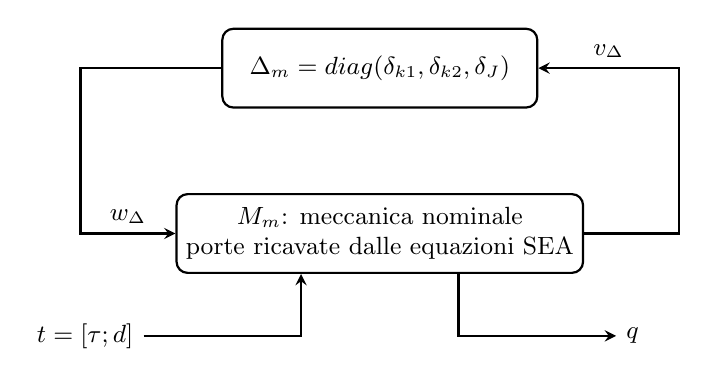
\begin{tikzpicture}[>=stealth,thick,every node/.style={font=\small},
 b/.style={draw,rounded corners,align=center,minimum width=4cm,minimum height=1cm}]
\node[b] (m) at (0,0) {$M_m$: meccanica nominale\\porte ricavate dalle equazioni SEA};
\node[b] (d) at (0,2.1) {$\Delta_m=\operatorname{diag}(\delta_{k1},\delta_{k2},\delta_J)$};
\draw[->] (m.east) -- (3.8,0) -- (3.8,2.1) -- node[above] {$v_\Delta$} (d.east);
\draw[->] (d.west) -- (-3.8,2.1) -- (-3.8,0) -- node[above] {$w_\Delta$} (m.west);
\draw[->] (-3,-1.3) node[left] {$t=[\tau;d]$} -- (-1,-1.3) -- (m.south -| -1,0);
\draw[->] (m.south -| 1,0) -- (1,-1.3) -- (3,-1.3) node[right] {$q$};
\end{tikzpicture}
